\documentclass[tikz,border=5pt]{standalone}
\usepackage{lmodern}
\usetikzlibrary{arrows.meta,positioning}

\begin{document}
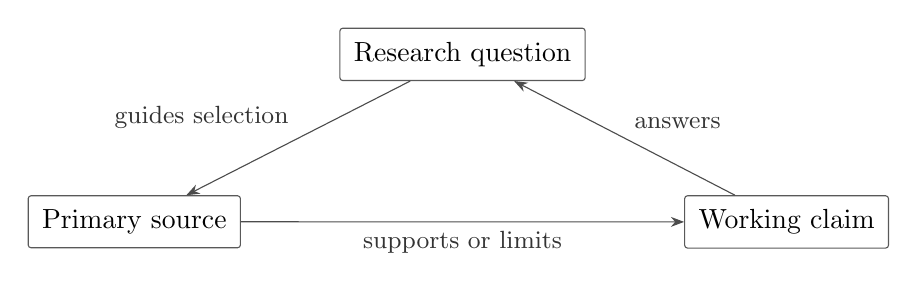
\begin{tikzpicture}[
  >=Stealth,
  concept/.style={draw=black!65,rounded corners=1pt,inner sep=5pt,align=center},
  relation/.style={font=\small,text=black!80},
]
  \node[concept] (question) {Research question};
  \node[concept,below left=1.45cm and 1.25cm of question] (source) {Primary source};
  \node[concept,below right=1.45cm and 1.25cm of question] (claim) {Working claim};
  \draw[->,black!70] (question) -- node[relation,above left] {guides selection} (source);
  \draw[->,black!70] (source) -- node[relation,below] {supports or limits} (claim);
  \draw[->,black!70] (claim) -- node[relation,above right] {answers} (question);
\end{tikzpicture}
\end{document}
